

\chapter{Methods}
\label{sec:Methods}



\section{Basic simulation techniques}
\label{sec:Basic simulation techniques}
% Simon

The basic molecular simulation techniques employed in \textit{ms}2 are well described in the literature \parencite{Allen, Frenkel, Rappaport} and are thus not repeated here. All non-standard methods that are implemented in \textit{ms}2 are introduced in section 5. The following paragraph briefly describes the most significant assumptions and
techniques employed in \textit{ms}2.

Simulations with \textit{ms}2 are performed in a quasi-infinite Cartesian space, using periodic boundary conditions \cite{born} and the minimum image convention \cite{metropolis}. The molecular interactions are considered to be pairwise additive, like in most other simulation packages. Including three- and many-body interactions leads to an increase in
computational effort while the benefits are questionable. As usual, the computational effort in \textit{ms}2 is reduced
by the introduction of a cut-off radius, up to which the intermolecular interactions are explicitly evaluated. The
contributions of interactions with molecules beyond the cut-off radius are accounted for by correction schemes.
For the electrostatic models, the reaction field method is included, while for the dispersive and repulsive interactions, a homogeneous fluid beyond the cut-off radius is assumed. The long range contributions are added to all
thermodynamic data that are calculated in \textit{ms}2.

Many thermodynamic properties calculated with \textit{ms}2 are residual quantities, indicated by the superscript "res".
To compare them to data that are measured on the macroscopic level, the solely temperature dependent contributions of the ideal gas have to be added. These ideal properties are accessible e.g. by quantum chemical methods
and can often be found in data bases \cite{rowley}.


The simulation program \textit{ms}2 internally uses reduced quantities for its calculations. All quantities are reduced by
a reference length $\sigma_{\text{R}}$, a reference energy $\epsilon_{\text{R}}$ and a reference mass $m_{\text{R}}$, respectively. These reference values are input variables and may, in principle, be chosen arbitrarily. However, it is recommended to use a reference length $\sigma_{\text{R}}$ in the order of 3 \AA, a reference energy $\epsilon_{\text{R}}/ k_{\text{B}}$ in the order of 100 K and a reference mass $m_{\text{R}}$ in the order of 50 atomic units. The reduction scheme for the most important physical quantities is listed in table~\ref{tab:ReductionScheme}. From these properties, the reduced form of all other quantities can be derived. An exception in the
reduction scheme is the chemical potential, which is normalized in \textit{ms}2 by $k_{\text{B}}T$ instead of $\epsilon_{\text{R}}$.
{\renewcommand{\arraystretch}{1.5}
	\begin{table}[h]
		\centering
		\caption{Important physical quantities in their reduced form. Note that $\epsilon_{0}$ indicates the permittivity of the vacuum $\epsilon_{0}=8.854187\times 10^{-12} \text{A}^{2}\text{s}^{4}\text{kg}^{-1}\text{m}^{-3}$.}
		\begin{tabular} [h] {ll@{=}l} 
			\hline \hline
			length & $l^{*}$ & $\frac{l}{\sigma_{\text{R}}}$ \\
			energy & $u^{*}$ & $\frac{u}{\epsilon_{\text{R}}}$ \\
			mass & $m^{*}$ & $\frac{m}{m_{\text{R}}}$\\ 
			time & $t^{*}$ & $\frac{t}{\sigma_{\text{R}}}\sqrt{\frac{\epsilon_{\text{R}}}{m_{\text{R}}}}$ \\
			piston mass & $Q^{*}_{\text{p}}$ & $\frac{Q_{\text{p}}\sigma_{\text{R}}^{4}}{m_{\text{R}}}$ \\
			temperature & $T^{*}$ & $\frac{Tk_{\text{B}}}{\epsilon_{\text{R}}}$ \\
			pressure & $p^{*}$ & $\frac{p\sigma_{\text{R}}^{3}}{\epsilon_{\text{R}}}$ \\
			density & $\rho^{*}$ & $\rho\sigma_{\text{R}}^{3}N_{\text{A}}$ \\                       
			volume & $V^{*}$ & $\frac{V}{\sigma_{\text{R}}^{3}}$ \\
			chemical potential & $\tilde{\mu}$ & $\frac{\mu}{k_{\text{B}}T}$ \\
			point charge & $q^{*}$ & $\frac{1}{\sqrt{4 \pi \epsilon_{0}}}\frac{q}{\sqrt{\epsilon_{\text{R}}\sigma_{\text{R}}}}$ \\
			dipole moment & $\mu^{*}$ & $\frac{1}{\sqrt{4 \pi \epsilon_{0}}}\frac{\mu}{\sqrt{\epsilon_{\text{R}}\sigma_{\text{R}}^{3}}}$ \\
			quadrupole moment & $Q^{*}$ & $\frac{1}{\sqrt{4 \pi \epsilon_{0}}}\frac{Q}{\sqrt{\epsilon_{\text{R}}\sigma_{\text{R}}^{5}}}$ \\
			diffusion coefficient & $D^{*}$ & $\frac{D}{\sigma\sqrt{m_{\text{R}}/ \epsilon_{\text{R}}}}$ \\
			viscosity & $\eta^{*}$ & $\frac{\eta \sigma_{\text{R}}^{2}}{\sqrt{m_{\text{R}} \epsilon_{\text{R}}}}$ \\
			thermal conductivity & $\lambda^{*}$ & $\frac{\lambda \sigma_{\text{R}}^{2}}{k_{\text{B}}\sqrt{m_{\text{R}} / \epsilon_{\text{R}}}}$ \\
			\hline \hline
			\addlinespace
		\end{tabular}   
		\label{tab:ReductionScheme}
	\end{table}
}


\section{Molecular Dynamics}
\label{sec:Molecular Dynamics}
% Simon 

Molecular dynamics (MD) meant to simulate the physical movements of particles (atoms, molecules, colloidal particles) of a given system. The path of the particles they follow through space as a function of time is determined from the forces acting between particles by numerically solving the Newton's equations of motion. These forces are described by atomistic force fields. Besides offering insight into molecular motion and providing direct structural information on an atomic scale MD allows to calculate macroscopic thermodynamic properties directly derived from the acting forces. In other words: we are able to obtain macroscopic properties from microscopic information. As MD follows the time evolution of the system, the outcome of a simulation is practically the time dependency of the calculated properties.




\subsection{Implemented Thermostat and Barostat}
\label{sec:Implemented Thermostat and Barostat}
% Simon 

In \textit{ms}2, two integrators are implemented to solve Newton's equations of motion during MD simulation: Leapfrog
and Gear predictor-corrector. These integrators are well known and described in literature \cite{allen}. The leapfrog
integrator is a second order integrator that requires little computational effort, while being robust for many applications. The error of the method scales quadratically with the length of the chosen time step. The Gear
predictor-corrector integrator is implemented with fifth order and is more accurate for small time steps compared to the Leapfrog integration \cite{allen}. The computational demand for both integration schemes is similar as
implemented in \textit{ms}2. The Gear integration, though being of higher order, is only 0.3\% slower than the Leapfrog
algorithm for the total calculation of one MD time step with a molecular model composed of three LJ sites,
having three rotational degrees of freedom. The thermostat incorporated in \textit{ms}2 is velocity scaling. Here, the velocities are scaled such that the actual kinetic energy matches the specified temperature. The scaling is applied equally over all molecular degrees of freedom. The pressure is kept constant using Andersen's barostat in MD, and random volume changes evaluated according to Metropolis acceptance criterion in MC, respectively.



\subsection{Integrators}
\label{sec:Integrators}
% Simon 




\section{Monte Carlo}
\label{sec:Monte Carlo}

The Monte Carlo (MC) method is the application of statistical mechanics to describe molecular systems. Problems that can be simulated with MC can also be modeled by the MD method. The difference is that the MC approach relies on statistics rather than trying to reproduce the trajectory of particles in real time. For MD the solution of Newton's equations of motion is the trajectory of every particle in the system, the trajectories can be interpreted as a sequence of states (configurations). The main idea behind MC is to create a set of configurations with Markov chain property such that this chain contains only relevant and physically meaningful configurations. In the standard MC simulation procedure, configurations of a given ensemble are generated in a stochastic way by performing trial (either temporary or permanent) changes in the system and then accepting them with an appropriate probability.


\subsection{Translation and rotation}
\label{sec:Moves}

For MC, independent on the choice of ensemble, the generation of trial configurations always includes at least molecular translational and rotational motions. Each new configuration generated by these moves is either rejected or accepted depending on the evaluation of its energy using a specific acceptance criterion. For an MC simulation, that has only molecular translational and rotational motions, one simulation step in $ms$2 is defined as \textit{the total number of molecular degrees of freedom in the system divided by 3} number of either translational or rotational attempts with randomly selected particles. In other words, during one step $N$ randomly selected molecules are both translated and rotated assuming the number of degrees of freedom for each molecules is 6, where $N$ is the number of molecules in the system.

\subsection{Resize}
\label{sec:Resize}

In an MC simulation, where the volume of the system does not remain constant, the creation of trial configurations also includes, next to molecular translational and rotational motions, the regular adjustment of the simulation volume. This is done by rescaling every intermolecular distance such that the relative distances between molecules along with their spatial orientations remain unchanged. In $ms$2, during one simulation step exactly one volume change attempt is made.

\section{Simulation Setup}
\label{sec:Simulation Setup}
% Simon 

\section{Interaction types}
\label{sec:Interaction types}

\subsection{Dispersive and Repulsive Interactions}
\label{sec:Dispersive and Repulsive Interaction}
% Minh 

In \textit{ms}2, the dispersive and repulsive interactions between molecules are reduced to pairwise interactions $u^{\text{LJ}}_{ij}$ of the different molecule sites $i$ and $j$, which are modeled by the 12-6-LJ potential \cite{lennard}
\begin{equation}
u^{\text{LJ}}_{ij}=4 \epsilon \left(\left(\frac{\sigma}{r_{ij}}\right)^{12}-\left(\frac{\sigma}{r_{ij}}\right)^{6}\right) \;.
\label{eq:DispersiveAndRepulsiveInteractions}
\end{equation}
Here, the site-site distance between two interacting LJ sites $i$ and $j$ is denoted by $r_{ij}$, while $\sigma$ and $\epsilon$ are the LJ size and energy parameters, respectively. The LJ potential is widely used and allows for a fast computation of these basic interactions. It has only two parameters, which facilitates the parameterization of molecular models.



\subsection{Electrostatic Interactions}
\label{sec:Electrostatic Interaction}
% Minh

\textit{ms}2 considers electrostatic interactions between electro-neutral molecules. Three different electrostatic site type
models are available: point charge, point dipole and linear point quadrupole. The two higher order electrostatic
interaction sites integrate characteristic arrangements of several single partial charges on a molecule. The simulative advantage of higher order polarities is faster execution and a better description of the electrostatic potential
of the molecule for a given number of electrostatic sites \cite{stone}. Combining two partial charges to one point dipole
reduces the computational effort with \textit{ms}2 by about 30\%, combining three point charges to one point quadrupole
reduces the computational demand by even 60\%. An additional advantage is the simplification of the molecular
model, which reduces the number of molecular model parameters. In the following, the implemented electrostatic interactions between sites of the same type and between unlike site types are briefly described.
\newline \newline
\textbf{Point charge.} Point charges are first order electrostatic interaction sites. The electrostatic interaction between
two point charges $q_{i}$ and $q_{j}$ is given by Coulomb's law \cite{allen}
\begin{equation}
u^{qq}_{ij}\left(r_{ij}, q_{i}, q_{j}\right)=\frac{1}{4 \pi \epsilon_{0}}\frac{q_{i}q_{j}}{r_{ij}} \;.
\label{eq:PointCharge}
\end{equation}
This interaction decays with the inverse of $r_{ij}$ and is therefore significant up to very large distances. For computational efficiency, the Coulombic contributions to the potential energy are explicitly evaluated up to a specified
cut-off radius $r_{\text{c}}$. The long range interactions with charges beyond $r_{\text{c}}$ are corrected for by the reaction field
method. Its application to point charges is discussed below.
\newline \newline
\textbf{Point dipole.} A point dipole describes the electrostatic field of two point charges with equal magnitude, but
opposite sign at a mutual distance $a \rightarrow 0$. Its moment $\mu$ is defined by $\mu=qa$. The electrostatic interaction
between two point dipoles with the moments $\mu_{i}$ and $\mu_{j}$ at a distance $r_{ij}$ is given by \cite{allen, gray}
\begin{equation}
u^{DD}_{ij}\left(r_{ij}, \theta_{i}, \theta_{j}, \phi_{ij}, \mu_{i}, \mu_{j}\right)=\frac{1}{4 \pi \epsilon_{0}}\frac{\mu_{i}\mu_{j}}{r_{ij}^{3}}\left(\sin \theta_{i} \sin \theta_{j} \cos \phi_{ij}-2 \cos \theta_{i} \cos \theta_{j}\right) \;,
\label{eq:PointDipole}
\end{equation}
with $\theta_{i}$ being the angle between the dipole direction and the distance vector of the two interacting dipoles and
$\phi_{ij}$ being the azimuthal angle of the two dipole directions, cf. Figure~\ref{fig:Schematic-of-the-angles}. In \textit{ms}2, the interaction between two dipoles is explicitly evaluated up to the specified cut-off radius $r_{\text{c}}$. The long range contributions are considered in \textit{ms}2 by the reaction field method \cite{allen}.
\begin{figure}[t]
	\centering
	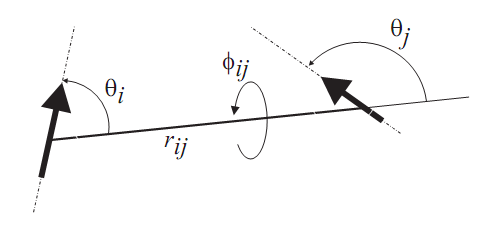
\includegraphics[width=0.55\columnwidth]{fig_Schematic-of-the-angles.png}
	\caption{Schematic of the angles between two point dipoles $i$ and $j$ indicated by the arrows, which are situated
		on different molecules at a distance $r_{ij}$.}
	\label{fig:Schematic-of-the-angles}
\end{figure}
\newline \newline
\textbf{Linear point quadrupole.} A linear point quadrupole describes the electrostatic field induced either by two
collinear point dipoles with the same moment, but opposite orientation at a distance $a \rightarrow 0$, or by at least
three collinear point charges with alternating sign $\left(q, -2q, q\right)$. The resulting quadrupole moment $Q$ is defined by $Q=2aq$. The electrostatic interaction between two linear point quadrupoles with the moments $Q_{i}$ and $Q_{j}$ at a
distance $r_{ij}$ is given by \cite{gray, hirschfelder}
\begin{eqnarray}
u^{QQ}_{ij}\left(r_{ij}, \theta_{i}, \theta_{j}, \phi_{ij}, Q_{i}, Q_{j}\right) & = & \frac{1}{4 \pi \epsilon_{0}}\frac{3}{4} \frac{Q_{i}Q_{j}}{r^{5}_{ij}} \nonumber \\ 
& & [1-5 (\left(\cos \theta_{i}\right)^2 + \left(\cos \theta_{j}\right)^{2}) - 15\left(\cos \theta_{i}\right)^{2}\left(\cos \theta_{j}\right)^{2}+ \nonumber \\ 
& & 2\left(\sin \theta_{i} \sin \theta_{j} \cos \phi_{ij} - 4 \cos \theta_{i} \cos \theta_{j}\right)^{2}] \;,
\end{eqnarray}
where the angles $\theta_{i}$, $\theta_{j}$ and $\phi_{ij}$ indicate the relative angular orientation of the two point quadrupoles, as discussed above. Note that no long range correction is necessary for this interaction type if the fluid is isotropic.
\newline \newline
\textbf{Point dipole interactions.} The interaction between a point dipole with moment $\mu_{i}$ and a point charge $q_{j}$ at a distance $r_{ij}$ is given by \cite{hirschfelder, lorrain}
\begin{equation}
u^{Dq}_{ij}\left(r_{ij}, \theta_{i}, \mu_{i}, q_{j}\right)=-\frac{1}{4\pi \epsilon_{0}} \frac{\mu_{i} q_{j}}{r^{2}_{ij}} \cos \theta_{i} \;.
\label{eq:PointDipoleInteractions}
\end{equation}
Here, $\theta_{i}$ is the angle between the distance vector of the point charge and the orientation vector of the point dipole, as illustrated in Figure~\ref{fig:Schematic-of-the-angles}.
\newline \newline
\textbf{Point quadrupole interactions.} The interaction potential of a linear point quadrupole $Q_{i}$ with a point charge $q_{j}$ at a distance $r_{ij}$ is given by \cite{allen, gray}
\begin{equation}
u^{Qq}_{ij}\left(r_{ij},\theta_{i},Q_{i},q_{j}\right)=\frac{1}{4\pi \epsilon_{0}} \frac{Q_{i}q_{j}}{4 r^{3}_{ij}}\left(3\cos^{2}\theta_{i}-1\right) \;,
\label{eq:PointQuadrupoleInteractionsPointCharge}
\end{equation}
where $\theta_{i}$ is the angle between the distance vector of the point charge and the orientation vector of the point
quadrupole, as illustrated in Figure~\ref{fig:Schematic-of-the-angles}.

The interaction between a linear point quadrupole with moment $Q_{i}$ and a point dipole with moment $\mu_{j}$ is given
by \cite{gray, hirschfelder}
\begin{eqnarray}
u^{Q\mu}_{ij}\left(r_{ij},\theta_{i},\theta_{j},\phi_{ij},Q_{i},\mu_{j}\right) & = & \frac{1}{4\pi\epsilon_{0}}\frac{3}{2}\frac{Q_{i}\mu_{j}}{r^{4}_{ij}}\left(\cos \theta_{i}-\cos \theta_{j}\right) \nonumber \\
& & \left(1+3\cos \theta_{i} \cos \theta_{j}-2\cos \phi_{ij} \sin \theta_{i} \sin \theta_{j}\right) \;,
\label{eq:PointQuadrupoleInteractionsPointDipole}
\end{eqnarray}
where the angles $\theta_{i}$, $\theta_{j}$ and $\phi_{ij}$ indicate the relative angular orientation of the point dipole $j$ and the point quadrupole $i$, as shown in Figure~\ref{fig:Schematic-of-the-angles}.
\newline \newline



\subsection{Intramolecular Interactions}
\label{sec:Intramolecular Interactions}
% Michael


\subsection{Mixing rules}
\label{sec:Mixing rules}
% Simon


For pure components, the interactions between two different LJ sites are described by the Lorentz-Berthelot
combination rules \cite{berthelot, lorentz}. For mixtures, the combination rules are extended to the modified Lorentz-Berthelot
rules, which include two additional parameters $\eta$ and $\xi$ to describe the interactions between LJ sites of unlike
molecules \cite{fischer}
\begin{eqnarray}
\sigma_{ij} &=& \eta\frac{\sigma_{i}+\sigma_{j}}{2} \;, \\
\epsilon_{ij} &=& \xi\sqrt{\epsilon_{i}\epsilon_{j}} \;.
\end{eqnarray}
The two parameters scale all LJ interactions between molecules of different components equally. Arbitrary
modifications of the combination rules are possible. \textit{ms}2 allows the specification of $\eta$ and $\xi$ for every molecule pair independently and thus the free parameterization of the combination rules.


\section{Cutoff \& long range correction}
\label{sec:Cutoff long range correction}
% 


\subsection{Reaction Field}
\label{sec:Reaction Field}
% 

\textbf{Reaction field method.} The truncation of interactions between first and second order electrostatic sites leads to
errors that need to be corrected. The reaction field method \cite{frenkel, nymand} is implemented in \textit{ms}2 for this task, being widely used and well accepted \cite{steinhauser, vanderSpoel}. Its advantages are accuracy and stability, while requiring little computational effort compared to other techniques like Ewald summation \cite{ewald}. However, it is limited to electro-neutral
systems, thus \textit{ms}2 is currently restricted to electro-neutral molecules. The basic assumption of the reaction field
method implemented in \textit{ms}2 is that the system is sufficiently large so that tinfoil boundary conditions $\left(\epsilon_{s} \rightarrow \infty\right)$
are applicable without a loss of accuracy. This is the case for $N\geq 500$ \cite{lisal, garzon, lisal1, jedlovszky}.

All dipoles within the cut-off radius $r_{\text{c}}$ polarize the fluid surrounding the cut-off sphere,
which is modeled as a dielectric continuum with a relative permittivity $\epsilon_{s}$. The polarization gives rise to a
homogeneous electric field within the cut-off radius, called the reaction field $\textbf{\textit{E}}^{\text{RF}}_{i}$ of magnitude
\begin{equation}
\textbf{\textit{E}}^{\text{RF}}_{i}=\frac{1}{4\pi \epsilon_{0}} \frac{2\left(\epsilon_{s}-1\right)}{2\epsilon_{s}+1} \frac{1}{r^{3}_{\text{c}}} \sum^{m}_{b=1} \sum_{j=1 \atop r_{ij}<r_{\text{c}}}^{N_{b}} \boldsymbol \mu_{b,j} \;.
\label{eq:ReactionFieldMethod}
\end{equation}
Note that all $m$ dipoles with moment $\boldsymbol \mu$ on all $N_{b}$ molecules within the cut-off sphere have to be summed up.
The reaction field acting outside of the cut-off sphere interacts with a dipole $\boldsymbol \mu_{i}$ at the center of the cut-off sphere by \cite{allen, boettcher}
\begin{equation}
u_{i}^{\mu \text{RF}}=- \frac{1}{2} \boldsymbol \mu_{i} \textbf{\textit{E}}_{i}^{\text{RF}} \;,
\label{eq:ReactionFieldMethodContribution}
\end{equation}
where $u_{i}^{\mu \text{RF}}$ is its contribution to the potential energy. Eq.~\eqref{eq:ReactionFieldMethodContribution} makes use of the assumption that the system is sufficiently large.

The reaction field method can also be applied to correct for sets of point charges, as long as they add up to a total
charge of zero. Therefore, a point charge distribution is reduced to a dipole vector $\boldsymbol \mu^{q}$ according to
\begin{equation}
\boldsymbol \mu^{q}=\sum^{n}_{i=1} \boldsymbol r_{i} q_{i} \;,
\label{eq:ReactionFieldMethodPointCharges}
\end{equation}
where $n$ denotes the total number of point charges and $\boldsymbol r_{i}$ the position vector of charge $q_{i}$. The resulting dipole $\boldsymbol \mu^{q}$ is transferred into the correction term according to Eqs.~\eqref{eq:ReactionFieldMethod} and~\eqref{eq:ReactionFieldMethodContribution}.


\subsection{Ewald summation}
\label{sec:Ewald summation}
% 

Ewald summation~\cite{allen1987, frenkel2003} was implemented for the calculation of electrostatic interactions between point charges. It extends the applicability of $ms$2 to thermodynamic properties of e.g. ions in solutions. In Ewald summation, the electrostatic interactions according to Coulomb's law are divided into two contributions: short-range and long-range. The short-range term includes all charge-charge interactions at distances smaller than the cut-off radius. The remaining contribution is calculated in Fourier space and only the final value is transformed back into real space. This allows for an efficient calculation of the long-range interactions between the charges. The algorithm is well described in literature. Currently, some of the new features, the calculation of Massieu potential derivatives and Hybrid MPI \& OpenMP Parallelization for MD, are not available together with Ewald summation.

% in ms2par ist auch "Rodgers" auswählbar!?!?

\section{Computing physical properties}
\label{sec:PhysProps}

\subsection{Ensembles Overview}
\label{sec:Ensembles}

An ensembles is the set of all theoretically possible configurations (states) under some specific macroscopic conditions. For example, the canonical ensemble ($NVT$) is the set of all configurations that fulfills the condition of having the same temperature $T$, volume $V$ and number of particles $N$, whereas the isobaric-isothermal ensemble ($NpT$) represents a system at constant temperature $T$, pressure $p$, and number of particles $N$. Independent on the specific macroscopic conditions, an MC simulation always involve the creation of a trial configuration according to some probability $\alpha_{ij}$, where $i$ refers to the previous state of the system, while $j$ refers to the new one generated with $\alpha_{ij}$ probability from $i$. Another probability, $a_{ij}$, determines that the newly generated state $j$ is actually accepted as a proper configuration of the specific ensemble or not. Thus, the transition probability between state $i$ and $j$ is $\pi_{ij}=\alpha_{ij} a_{ij}$. The transition probability for state $i$ depends only on the previous state $j$. This property is called the Markov chain property; the sequence of configurations created by this way is defined as the Markov chain. It can be shown that if a Markov chain satisfies the condition $P_i \pi_{ij}=P_j \pi_{ji}$ (for every state $i$ and $j$) of \textit{microscopic reversibility} then the probability of every configuration in the Markov chain will converge to the arbitrarily chosen set of probabilities $\textbf{P}=[P_1,P_2,...,P_i,...]$ as the length of the chain increases. Once \textbf{P} is specified, the microscopic reversibility condition $P_i \pi_{ij}=P_j \pi_{ji}$ can be solved and has potentially more than one solution for $a_{ij}$. A solution for $a_{ij}$ is called the acceptance criterion of the ensemble. The generation of the next potential configuration is done such a way that $\alpha$ is symmetric, i.e. $\alpha_{ij}=\alpha_{ji}$. This way $\alpha_{ij}$ and $\alpha_{ji}$ cancel each other in the equation. It is sensible to specify $\textbf{P}=[P_1,P_2,...,P_i,...]$ as the set of actual probability of occurrence of the configurations $1,2,...,i,...$ in the ensemble.\\
With the exception of the $NVE$ ensemble, not every theoretically possible configuration of an ensemble has the same probability of occurrence. In fact, only a small subset of configurations is truly relevant even though the set of all theoretically possible configurations of an ensemble is extremely large. Although, the analytical form of $P_i$ is known for an ensemble, its numerical value is not. Therefore, the way of calculating a macroscopic property $A$ as an \textit{ensemble average} using the standard statistical formula for the expected value $<A>=\sum A_i P_i$ (for every possible $i$), where $A_i$ is the value of property $A$ for configuration $i$, is not feasible. However, it can be shown that if configurations are selected randomly (\textit{Monte Carlo sampling}) and selected according to their actual probability of occurrence $P_i$ at the same time (\textit{importance sampling}) then the expected value can be calculated as $<A>=\sum A_i/n$ (assuming the number of sampled configurations $n$ is large enough). A Markov chain satisfying the microscopic reversibility criterion $P_i \pi_{ij}=P_j \pi_{ji}$ fulfills exactly this condition, because it selects $n$ configurations according to their actual probability of occurrence $P_i$.
 
Following type of simulations are currently supported by \textit{ms}2:
\begin{itemize}
	\item canonical ensemble ($NVT$) MC (corresponds to MD with thermostat)
	\item micro-canonical ensemble ($NVE$) MC (corresponds to MD)
	\item isobaric-isothermal ensemble ($NpT$) MC (corresponds to MD with thermostat and barostat)
	\item grand equilibrium method (pseudo-$\mu VT$) MC (MC only)
\end{itemize}

For the micro-canonical ensemble, the MC acceptance criterion for molecular translation and rotation is 
\begin{equation}
\mathrm{min}\left(1, \frac{(E-U_j)^{(F-2)/2} \mathrm{\theta(E-U_j)}}{(E-U_i)^{(F-2)/2} \mathrm{\theta(E-U_i)}} \right) ,
\label{eq:acccritNVE}
\end{equation}
where $E$ is the total \textit{hamiltonian} of the system that is a sum of the total kinetic $K$ and potential energy $U$ of the system, $F$ is the sum of the individual molecular degrees of freedom in the system, and $\theta$ is the unit step function \cite{Lus98}.
The MC acceptance criterion for the canonical ensemble for molecular translation and rotation is 
\begin{equation}
\mathrm{min}\left(1, \mathrm{exp}(-\beta(U_j-U_i)) \right),
\label{eq:acccritNVT}
\end{equation}
where $\beta$ is the inverse temperature.\\

For the $NpT$ ensemble, the MC acceptance criterion for molecular translation and rotation as well as volume change is
\begin{equation}
\text{min}\left(1, \text{exp}( -\beta(U_j-U_i+p(V_j-V_i))+N\text{ln}(V_j/V_i) )  \right).
\label{eq:acccritNVT}
\end{equation}

\subsection{Statistical uncertainties}
\label{sec:Statun}

The simulation program \textit{ms}2 calculates the thermodynamic properties from the trajectories (MD) or Markov Chains (MC) on the fly. The results are written to file with a specified frequency during the course of the simulation. The statistical uncertainties of all results are estimated using the block averaging method according to Flyvbjerg and Petersen \cite{flyvberg} and the error propagation law.

\subsection{Static properties from Helmholtz free energy derivatives (NVT, NVE)}
\label{sec:PropHelm}

Standard textbook approaches in the molecular simulation literature indicate specific statistical mechanical ensembles for particular thermodynamic properties. E.g., properties originating from differentiation with respect to temperature at constant pressure, such as the isothermal compressibility, are most likely considered to be candidates for the $NpT$ ensemble, while for a property such as the isochoric heat capacity, the $NVT$ ensemble is considered to be a natural choice. It is true that certain properties have simpler statistical analogs in certain ensembles and may be difficult to derive in other ensembles. Fundamentally, however, the above mentioned philosophy misleading. In principle, any thermodynamic property is accessible in any ensembles. The formalism proposed by Lustig ~\cite{Lus11, Lus12} allows for the calculation of an arbitrary number of derivatives
\begin{align} 
A^\mathrm{r}_{nm}=(1/T)^n \rho^m \frac{\partial^{n+m}f^\text{r}(T,\rho)/(RT)}{\partial(1/T)^n \partial \rho^m}
\label{eq:helmholtzderiv}
\end{align}
for $n>0$ or $m>0$ in the $NVT$ and $NVE$ ensembles, with the molar residual Helmholtz energy $f$, the temperature $T$, the density $\rho$, the molar gas constant $R$. It can be shown that the total $f/(RT)$ can be additively separated into an ideal $f^\text{o}/(RT)$ and a residual part$f^\text{r}/(RT)$. The ideal part by definition corresponds to the value of $f/(RT)$ when no intermolecular interactions are at work \cite{SpanBook}. $f^\text{o}/(RT)$ consist of an exclusively temperature and an exclusively density dependent part. The former has a trivial density dependence $\ln(\rho/\rho_\text{ref})$, whereas the latter has a non-trivial temperature dependence.\\
The approach is based on the fact that the fundamental equation of state contains the complete thermodynamic information about a system, which can be expressed in terms of various thermodynamic potentials~\cite{MunsterBook}, e.g. internal energy $E(N,V,S)$, enthalpy $H(N,p,S)$, Helmholtz free energy $F(N,V,T)$ or Gibbs free energy $G(N,p,T)$, with number of particles $N$, volume $V$, pressure $p$, temperature $T$ and entropy $S$. These representations are equivalent in the sense that any other thermodynamic property is essentially a combination of derivatives of the chosen form with respect to its independent variables. The form $f/(RT)(N,V,1/T)$, known as the Massieu potential, is preferable due to practical reasons. Namely, neither its independent variables nor its derivatives with respect these variables involve entropic properties. Moreover, some of its derivatives are directly related to measurable properties.\\
Since $f$ is a thermodynamic potential, any other static thermodynamic property is a combination of its partial derivatives. The molar internal energy $u$, pressure $p$, molar enthalpy $h$, molar Gibbs energy $g$, and molar isochoric heat capacity $c_v$ are simple functions
\begin{align}
\frac{u}{RT}=A^\text{o}_{10}(T)+A^\text{r}_{10},
\label{eq:internalen}
\end{align}
\begin{align}
\frac{p}{\rho RT}=1+A^\text{r}_{01},
\label{eq:pressure}
\end{align}
\begin{align}
\frac{1}{RT}\left(\frac{\partial p}{\partial \rho}\right)_T=1+2A^\text{r}_{01}+A^\text{r}_{02},
\label{eq:dpdrho}
\end{align}
\begin{align}
\frac{1}{\rho{R}}\left(\frac{\partial p}{\partial T}\right)_\rho=1+A^\text{r}_{01}-A^\text{r}_{11},
\label{eq:dpdt}
\end{align}
\begin{align}
\frac{h}{RT}=1+A^\text{r}_{01}+A^\text{o}_{10}(T)+A^\text{r}_{10},
\label{eq:enthalpy}
\end{align}
\begin{align}
\frac{g}{RT}=1+A^\text{r}_{01}+A^\text{o}_{00}+A^\text{r}_{00},
\label{eq:gibbs}
\end{align}
\begin{align}
\frac{c_v}{R}=-A^\text{o}_{20}(T)-A^\text{r}_{20},
\label{eq:cv}
\end{align}
while molar isobaric heat capacity $c_p$, and speed of sound $w$ are non-linear combinations of derivatives
\begin{align}
\frac{c_p}{R}=-A^\text{o}_{20}(T)-A^\text{r}_{20}+\frac{(1+A^\text{r}_{01}-A^\text{r}_{11})^2}{1+2A^\text{r}_{01}+A^\text{r}_{02}},
\label{eq:cp}
\end{align}
\begin{align}
\frac{Mw^2}{RT}=1+2A^\text{r}_{01}+A^\text{r}_{02}-\frac{(1+A^\text{r}_{01}-A^\text{r}_{11})^2}{A^\text{o}_{20}(T)+A^\text{r}_{20}},
\label{eq:sos}
\end{align}
where $M$ is the molar mass, $A^\text{r}_{nm}=A^\text{r}_{nm}(T, \rho)$, and $A^\text{o}_{nm}=A^\text{o}_{nm}(T, \rho)=(1/T)^n \rho^m \cdot \partial^{n+m}[\alpha^\text{o}(T)+\alpha^\text{o}(\rho)]/\partial(1/T)^n / \partial \rho^m =A^\text{o}_{nm}(T)+A^\text{o}_{nm}(\rho)$. Note that the ideal part
\begin{itemize}
	\item $A^\text{o}_{nm}(T, \rho)=0$, for $n>0$ and $m>0$,
	\item $A^\text{o}_{nm}(T, \rho)=A^\text{o}_{nm}(T)+0$, for $n>0$ and $m=0$,
	\item $A^\text{o}_{nm}(T, \rho)=0+(-1)^{1+m}$, for $n=0$ and $m>0$.
\end{itemize}
A more complete list of thermodynamic properties can be found in Ref. \cite{SpanBook}. For the $NVE$ ensemble, there are two sets of $A^\text{r}_{nm}$ output values in $ms$2. Each set corresponds to a different statistical mechanical entropy definition \cite{Lus12}. The numerical values for these definitions should converge to the same number as the system size increases and they should be identical in the thermodynamic limit $(N \rightarrow \infty)$.\\

The $A^\text{r}_{nm}$ derivatives are determined from fluctuation formulas. These fluctuation formulas require the ensemble average of $U^n$ and ${\partial^m U}/{\partial V^m}$ with respect to the applied molecular interaction pair potential. Thus the explicit analytical expressions for $U^n$ and ${\partial^m U}/{\partial V^m}$ have to be determined analytically beforehand ~\cite{Lus11, Lus12}. The general formula for ${\partial^m U}/{\partial V^m}$ can be found in Ref. ~\cite{Lus94b}. For common molecular interaction pair potentials, like the Lennard-Jones potential~\cite{allen}, describing repulsive and dispersive interactions, or Coulomb's law, describing electrostatic interactions between point charges, the explicit analytical formulas can be obtained straightforwardly. The mathematical form of the long range correction (LRC) for $U$ and ${\partial^m U}/{\partial V^m}$ depends on the molecular interaction potential and the cut-off method (site-site or center-of-mass cut-off mode) applied. For the Lennard-Jones potential, the LRC scheme was well described in the literature for both the site-site~\cite{Lus11, Mei06} and the center of mass cut-off mode~\cite{Lus94b, Lus88}. For the usual implementation of the reaction field method ~\cite{RFmethod, siteRFmethod}, the LRC for ${\partial^m U}/{\partial V^m}$ can be obtained straightforwardly. However, practical applications show that the electrostatic LRC of ${\partial U}/{\partial V}$ and ${\partial^2 U}/{\partial V^2}$ can be neglected in case of systems for which the reaction field method is an appropriate choice. E.g., the contribution of the electrostatic LRC for a liquid system ($T=298$ K and $\rho= 45.86$ mol/l) consisting of only 200 water and 50 methanol molecules with a very short cut-off radius of $20\%$ of the edge length of the simulation volume is still $<<1\%$ for both ${\partial U}/{\partial V}$ and ${\partial^2 U}/{\partial V^2}$.\\

The supplementary material of Ref. ~\cite{ms2release2.0} contains the explicit fluctuation formulas as well as the LRC contributions with respect to the implemented molecular interaction pair potentials in $ms$2 for the $A^\text{r}_{nm}$ derivatives up to the order of $n=3$ and $m=2$.

\subsection{Static properties from conventional fluctuation formulas (NpT, NpH)}
\label{sec:PropConv}

Several static thermodynamic properties have simple statistical analogs in certain ensembles.\\

%At constant temperature and volume ($NVT$ ensemble), e.g. the pressure is determined by the virial expression $W$. Other important
%thermodynamic properties are accessible at constant temperature and pressure. In the $NpT$ ensemble, the volume is a fluctuating %parameter that on average yields the volume corresponding to the specified temperature and
%pressure. In both ensembles, the residual internal energy is the sum of all pairwise interaction energies $u_{ij}$ and
%the appropriate long range correction. The residual enthalpy is linked to the residual internal energy, pressure
%and volume of the system using the thermodynamic definition.

%At constant temperature $T$ and volume $V$, the pressure $p$ is determined by \cite{allen}
%\begin{equation}
%p=\frac{k_{\text{B}}T}{V}+\frac{\left\langle W\right\rangle}{V}+\Delta p^{L}=\frac{k_{\text{B}}T}{V}+\frac{1}{3V}\left\langle %\sum^{N-1}_{i=1}\sum_{j=i+1\atop r_{ij}<r_{\text{c}}}^{N} \textbf{\textit{r}}_{ij}\textbf{\textit{f}}_{ij}\right\rangle +\Delta %p^{L} \;,
%\label{eq:pressure}
%\end{equation}
%where $k_{\text{B}}$ is the Boltzmann constant and the brackets $\left\langle \ldots \right\rangle$ indicate the ensemble average. $W$ denotes the virial,
%which is defined by the force vector $\textbf{\textit{f}}_{ij}$ acting between two molecules at a separation vector %$\textbf{\textit{r}}_{ij}$ between their centers of mass. The contribution $\Delta p^{L}$ considers the long-range interactions with %molecules beyond the cut-off radius $r_{\text{c}}$.

%In the $NpT$ ensemble, the volume is a fluctuating parameter that on average yields the volume
%corresponding to the specified pair of temperature $T$ and pressure $p_{0}$. In MD simulations with Andersen's
%barostat \cite{andersen}, which is implemented in \textit{ms}2, the fluctuations of the volume are damped by a fictive piston mass %$Q_{\text{p}}$ according to the equation of motion
%\begin{equation}
%\ddot{V}=\frac{p-p_{0}}{Q_{\text{p}}} \;.
%\label{eq:fictivepistonmass}
%\end{equation}
%In MC simulations, the volume is changed randomly and the new volume accepted by applying the Metropolis
%acceptance criterion
%\begin{equation}
%P_{acc}=\text{min} \left(1, \exp \left(\frac{\Delta E}{k_{\text{B}}T}\right)\right) \;,
%\label{eq:metropolisacceptancecriterion}
%\end{equation}
%where $P_{acc}$ is the probability of accepting the volume change and $\Delta E$ is the difference between the old state with
%energy $U_{old}$ for the volume $V_{old}$ and the new state with energy $U_{new}$ for the volume $V_{new}$ according to
%\begin{equation}
%\Delta E=p_{0}\left(V_{new}-V_{old}\right)+\left(U_{new}-U_{old}\right)+Nk_{\text{B}}T \ln \frac{V_{old}}{V_{new}} \;.
%\label{eq:differencestate}
%\end{equation}

%The residual enthalpy $H^{\text{res}}$ is directly linked to the residual internal energy, pressure and volume of the system
%\begin{equation}
%H^{\text{res}}=U^{\text{res}}+pV-Nk_{\text{B}}T \;,
%\label{eq:enthalpy}
%\end{equation}
%where $U^{\text{res}}$ is the residual potential energy. It is defined as the sum of all pairwise interaction energies $u_{ij}$ and
%the appropriate long range correction $\Delta U^{L}$, cf. section 5.5
%\begin{equation}
%U^{\text{res}}=\sum^{N-1}_{i=1} \sum_{j=i+1\atop r_{ij}<r_{\text{c}}}^{N} u_{ij} + \Delta U^{L} \;.
%\label{eq:internalenergy}
%\end{equation}


%The accessible second derivatives vary with the employed ensemble. In the $NVT$ ensemble, the residual
%isochoric heat capacity $c^{res}_{v}$ is determined by fluctuations of the residual potential energy $U^{\text{res}}$
%\begin{equation}
%c^{\text{res}}_{v}=\frac{1}{N} \left(\frac{\partial U^{\text{res}}}{\partial %T}\right)_{v}=\frac{1}{k_{\text{B}}\left(NT\right)^{2}}\left(\left\langle \left(U^{\text{res}}\right)^{2}\right\rangle - %\left\langle U^{\text{res}}\right\rangle ^{2}\right) \;.
%\label{eq:isochoricheatcapacity}
%\end{equation}
%The partial derivative of the potential energy with respect to the volume at constant temperature $(\partial U^{\text{res}}/ %\partial V)_{T}$ is determined by fluctuations of the residual potential energy $U^{\text{res}}$ and the virial $W$
%\begin{equation}
%\left(\frac{\partial U^{\text{res}}}{\partial V}\right)_{T}=\frac{N}{3V} \left(\frac{1}{k_{\text{B}}T}\left(\left\langle %W\right\rangle \left\langle U^{\text{res}}\right\rangle - \frac{1}{N} \left\langle WU^{\text{res}}\right\rangle\right)+\left\langle %W\right\rangle \right) \;.
%\label{eq:partialderivativeofthepotentialenergy}
%\end{equation}

In the $NpT$ ensemble, the second derivatives of the Gibbs energy, namely the residual isobaric heat capacity $c^{\text{res}}_{p}$, the isothermal compressibility $\beta_{T}$ and the volume expansivity $\alpha_{p}$ are functions of ensemble fluctuations \cite{allen}. The residual isobaric heat capacity $c^{\text{res}}_{p}$ is related to fluctuations of the residual enthalpy $H^{\text{res}}$
\begin{equation}
c^{\text{res}}_{p}=\frac{1}{N} \left(\frac{\partial H^{\text{res}}}{\partial T}\right)_{p} = \frac{1}{k_{\text{B}}\left(NT\right)^{2}} \left(\left\langle \left(H^{\text{res}}\right)^{2}\right\rangle-\left\langle H^{\text{res}}\right\rangle ^{2}\right) \;.
\label{eq:isobaricheatcapacity}
\end{equation}
To obtain the total isobaric heat capacity $c_{p}$, the solely temperature dependent ideal gas contribution $c^{\text{id}}_{p}\left(T\right)$ has to be added. This ideal property is accessible e.g. by quantum chemical methods and can often be found in data bases \cite{rowley}.

An analogous relationship links the isothermal compressibility $\beta_{T}$ to volume fluctuations in the $NpT$ ensemble
\begin{equation}
\beta_{T}=-\frac{1}{V}\left(\frac{\partial V}{\partial p}\right)_{T}=\frac{1}{k_{\text{B}}T\left\langle V\right\rangle} \left(\left\langle V^{2}\right\rangle - \left\langle V\right\rangle ^{2}\right) \;.
\label{eq:isothermalcompressibility}
\end{equation}
The partial derivative of the residual enthalpy with respect to the pressure at constant temperature $(\partial H^{\text{res}}/ \partial p)_{T}$ is linked to fluctuations of volume and residual internal energy
\begin{equation}
\left(\frac{\partial H^{\text{res}}}{\partial p}\right)_{T}=V-\frac{N}{T}\left(\left\langle U^{\text{res}}V\right\rangle - \left\langle U^{\text{res}}\right\rangle\left\langle V\right\rangle+p\left(\left\langle V^{2}\right\rangle-\left\langle V\right\rangle ^{2}\right)\right) \;,
\label{eq:derivativeoftheresidualenthalpy}
\end{equation}
and the volume expansivity $\alpha_{p}$ again to volume and residual enthalpy fluctuations
\begin{equation}
\alpha_{p}=\frac{1}{V}\left(\frac{\partial V}{\partial T}\right)_{p}=\frac{N}{T^{2}\left\langle V\right\rangle}\left(\left\langle H^{\text{res}}V\right\rangle-\left\langle H^{\text{res}}\right\rangle\left\langle V\right\rangle\right) \;.
\label{eq:volumeexpansivity}
\end{equation}

The speed of sound $w$ is the velocity of a sound wave traveling through an elastic medium. It can be given by the
isothermal compressibility $\beta_{T}$, the volume expansivity $\alpha_{p}$, the isobaric heat capacity $c_{p}$ and the temperature $T$ by
\begin{equation}
w=\left(\frac{1}{M\left(\beta_{T}\rho-T\alpha^{2}_{p}/c_{p}\right)}\right)^{0.5} \;,
\label{eq:speedofsound}
\end{equation}
where $M$ is the molar mass. In \textit{ms}2, the speed of sound is calculated both for pure components and mixtures in the $NpT$ ensemble.

\subsection{Transport properties}
\label{sec:Transport properties}
% Tatjana

In \textit{ms}2, transport properties are calculated using equilibrium MD. Here, the fluctuations of a system around
its equilibrium state are evaluated as a function of time. The Green-Kubo formalism relates these microscopic
fluctuations to the respective transport properties.
\newline \newline
\textbf{Diffusion coefficients.} The self-diffusion coefficient $D_{i}$ is related to the mass flux of single molecules within a fluid. Therefore, the relevant Green-Kubo expression is based on the individual molecule velocity autocorrelation
function \cite{gubbins1}
\begin{equation}
D_{i}=\frac{1}{3N_{i}}\int^{\infty}_{0} \mathrm dt \left\langle \textbf{v}_{k}\left(t\right) \cdot \textbf{v}_{k}\left(0\right)\right\rangle \;,
\label{eq:selfdiffusioncoefficient}
\end{equation}
where $\textbf{v}_{k}\left(t\right)$ is the center of mass velocity vector of molecule $k$ at some time $t$. Eq.~\eqref{eq:selfdiffusioncoefficient} is an average over all $N_{i}$ molecules of component $i$ in the ensemble, since all contribute to the self-diffusion coefficient. In binary mixtures, the Maxwell-Stefan diffusion coefficient $\dcoeff_{ij}$ is defined by \cite{krishna}
\begin{equation}
\dcoeff_{ij}=\frac{x_{j}}{x_{i}}\Lambda_{ii}+\frac{x_{i}}{x_{j}}\Lambda_{jj}-\Lambda_{ij}-\Lambda_{ji} \;,
\label{eq:diffusioncoefficient}
\end{equation}
where $x_{i}=N_{i}/N$ and $\Lambda_{ij}$ can be written in terms of the center of mass velocity
\begin{equation}
\Lambda_{ij}=\frac{1}{3N} \int^{\infty}_{0} \mathrm dt \left\langle \sum^{N_{i}}_{k=1} \textbf{v}_{i,k}\left(0\right) \cdot \sum^{N_{j}}_{l=1} \textbf{v}_{j,l} \left(t\right)\right\rangle \;.
\label{eq:difcoef}
\end{equation}
From the expressions above, the collective character of the Maxwell-Stefan diffusion coefficient is evident. This
leads to significantly less data for a given system size and time step and therefore to larger statistical uncertainties
than in case of the self-diffusion coefficient. Note that equations for the Maxwell-Stefan diffusion coefficient are
implemented in \textit{ms}2 both for binary and ternary mixtures \cite{krishna}.
\newline \newline
\textbf{Shear viscosity.} The shear viscosity $\eta$, as defined by Newton's "law" of viscosity, is a measure of the resistance of a fluid to a shearing force \cite{hoheisel}. It is associated with the momentum transport under the influence of velocity
gradients. Hence, the shear viscosity can be related to the time autocorrelation function of the off-diagonal
elements of the stress tensor $\textbf{J}_{p}$ \cite{gubbins1}
\begin{equation}
\eta=\frac{1}{Vk_{\text{B}}T} \int^{\infty}_{0} \mathrm dt \left\langle J^{xy}_{p}\left(t\right) \cdot J^{xy}_{p}\left(0\right)\right\rangle \;.
\label{eq:shearviscosity}
\end{equation}
Averaging over all three independent elements of the stress tensor, i.e. $J^{xy}_{p}$, $J^{xz}_{p}$ and $J^{yz}_{p}$, improves the statistics.
The component $J^{xy}_{p}$ of the microscopic stress tensor $\textbf{J}_{p}$ is given in terms of the molecular positions and velocities by \cite{hoheisel}
\begin{equation}
J^{xy}_{p}=\sum^{N-1}_{i=1} mv^{x}_{i}v^{y}_{i}-\sum^{N-1}_{i=1}\sum^{N}_{j=i+1}\sum^{n}_{k=1}\sum^{n}_{l=1} r^{x}_{ij} \frac{\partial u_{ij}}{\partial r^{y}_{kl}} \;.
\label{eq:componentofstresstensor}
\end{equation}
Here, the lower indices $l$ and $k$ indicate the $n$ interaction sites of a molecule and the upper indices $x$ and $y$ denote
the spatial vector components, e.g. for velocity $v^{x}_{i}$ or site-site distance $r^{x}_{ij}$. The first term of Eq.~\eqref{eq:componentofstresstensor} is the kinetic energy contribution and the second term is the potential energy contribution to the shear viscosity. Consequently, the Green-Kubo integral~\eqref{eq:shearviscosity} can be decomposed into three parts, i.e. the solely kinetic energy contribution, the solely potential energy contribution and the mixed kinetic-potential energy contribution \cite{hoheisel}.
\newline \newline
\textbf{Bulk viscosity.} The bulk viscosity $\eta_{v}$ refers to the resistance to dilatation of an infinitesimal volume element at constant shape \cite{barton}. The bulk viscosity can be calculated by integration of the time-autocorrelation function
of the diagonal elements of the stress tensor and an additional term that involves the product of pressure $p$ and
volume $V$, which does not appear in the shear viscosity, cf. Eq.~\eqref{eq:shearviscosity}. In the $NVE$ ensemble, the bulk viscosity
is given by \cite{gubbins1, steele}
\begin{equation}
\eta_{v}=\frac{1}{Vk_{\text{B}}T} \int^{\infty}_{0} \mathrm dt \left\langle \left(J^{xx}_{p}\left(t\right)-pV\left(t\right)\right) \cdot \left(J^{xx}_{p}\left(0\right)-pV\left(0\right)\right)\right\rangle \;.
\label{eq:bulkviscosity}
\end{equation}
The diagonal component $J^{xx}_{p}$ of the microscopic stress tensor $\textbf{J}_{p}$ is defined analogous to Eq.~\eqref{eq:componentofstresstensor}. The statistics of the ensemble average in Eq.~\eqref{eq:bulkviscosity} can be improved using all three independent diagonal elements of the stress
tensor $J^{xx}_{p}$, $J^{yy}_{p}$ and $J^{zz}_{p}$. Eqs.~\eqref{eq:componentofstresstensor} and~\eqref{eq:bulkviscosity} can directly be applied for mixtures.

\textbf{electric conductivity}
The evaluation of the electric conductivity $\sigma$ was implemented in $ms$2 version 2.0, being a measure for the flow of ions in solution. The Green-Kubo formalism~\cite{gubbins1972} offers a direct relationship between $\sigma$ and the time-autocorrelation function of the electric current flux $\bm{j_e}(t)$ ~\cite{HansenBook}
\begin{equation}
\sigma=\frac{1}{3Vk_{\mathrm{B}}T}\int_0^{\infty}~\big\langle \bm{j_e}(t)\cdot \bm{j_e}(0) \big\rangle  \mathrm{d} t \mbox{   ,}
\label{Erdalkali_elcond}
\end{equation}
where $k_\texttt{B}$ is Boltzmann’s constant. The electric current flux is defined by the charge $q_k$ of ion $k$ and its velocity vector $\bm{v}_k$ according to
\begin{equation}
\bm{j_e}(t)=\sum_{k=1}^{N_{j}} q_k \cdot \bm{v}_{k}(t) \mbox{   ,}
\label{elflux}
\end{equation}
where $N_{j}$ is the number of molecules of component $j$ in solution. Note that only the ions in the solution have to be considered, not the electro-neutral molecules.
For better statistics, $\sigma$ is sampled over all independent spatial elements of $\bm{j_e}(t)$.



\textbf{thermal conductivity}
In the previous version of $ms2$ the determination of the thermal conductivity by means of the Green-Kubo formalism was implemented for pure substances only. In the present release, the calculation of the thermal conductivity was extended to multi-component mixtures. The thermal conductivity $\lambda$ is given by the autocorrelation function of the elements of the microscopic heat flow ${J}^{x}_{q}$
\begin{equation}\label{themalcond}
\lambda=\frac{1}{Vk_BT^{2}}\int_{0}^{\infty} dt~\big\langle {J}^x_q(t)\cdot {J}^x_q(0)\big\rangle.
\end{equation}
\noindent In mixtures, energy transport and diffusion occur in a coupled manner, thus, the heat flow for a mixture of $n$ components is given by~\cite{evans1}
\begin{eqnarray}
\mathbf{J}_q &=& \frac{1}{2} \sum_{i=1}^{n} \sum_{k=1}^{N_i}\left[ m_{i}^{k}\left({v}_{i}^{k}\right)^2+ \nonumber
\mathbf{w}_i^k \mathbf{I}_i^k \mathbf{w}_i^k+\sum_{j=1}^{n}\sum_{l \neq k}^{N_j} u\left(r_{ij}^{kl}\right)\right]\cdot \mathbf{v}_i^k \\
& -&\frac{1}{2}\sum_{i=1}^{n} \sum_{j=1}^{n} \sum_{k=1}^{N_i} \sum_{l \neq k}^{N_j} \bm{r}_{ij}^{kl}\cdot
\big( \mathbf{v}_i^k \cdot \frac{\partial u\left(r_{ij}^{kl}\right)}{\partial \bm{r}_{ij}^{kl}}+\mathbf{w}_i^k \mathbf{\Gamma}_{ij}^{kl}\big)- \sum_{i=1}^{n} h_{i}\sum_{k=1}^{N_i} \mathbf{v}_{i}^{k}\mbox{   ,}\label{heatflow} 
\end{eqnarray}
\noindent where $\mathbf{w}^k_i$ is the angular velocity vector of molecule $k$ of component $i$ and $\mathbf{I}^k_i$ its matrix of angular momentum of inertia. $u\left(r_{ij}^{kl}\right)$ is the intermolecular potential energy and $\mathbf{\Gamma}_{ij}^{kl}$ is the torque due to the interaction of molecules $k$ and $l$. The indices $i$ and $j$ denote the components of the mixture. $h_{i}$ is the partial molar enthalpy. It has to be specified as an input in the $ms2$ parameter file and can be calculated from $NpT$ simulations.



\subsection{radial distribution function}
\label{sec:radial distribution function}
% Tatjana / Simon

The \textbf{radial distribution} function (RDF) $g(r)$ is a measure for the microscopic structure of matter. It is defined by the local number density around a given position within a molecule $\rho^L(r)$ in relation to the overall number density $\rho = N/V$

\begin{equation} g(r) = \dfrac{\rho^L(r)}{\rho} = \dfrac{1}{\rho}\dfrac{\mathrm{d}N(r)}{\mathrm{d}V} = \dfrac{1}{4 \pi r^2 \rho} \dfrac{\mathrm{d}N(r)}{\mathrm{d}r}. \label{Eq:gr} \end{equation}
Therein, $\mathrm{d}N(r)$ is the differential number of molecules in a spherical shell volume element $\mathrm{d}V$, which has the width $\mathrm{d}r$ and is located at the distance $r$ from the regarded position. $g(r)$ can be evaluated for every molecule of a given species. 

In the present release of $ms$2, the RDF can be calculated during MD simulation runs for pure components and mixtures on the fly. The RDF is sampled between all LJ sites. In order to evaluate RDFs for arbitrary positions, say point charge sites, superimposed dummy LJ sites with the parameters $\sigma = \epsilon = 0$ have to be introduced in the potential model file by the user.


The \textbf{residence time} $\tau_{j}$ defines the average time span that a molecule of component $j$ remains within a given distance $r_{ij}$ around a specific molecule $i$. It is given by the autocorrelation function
\begin{equation}
\tau_{j} = \int_{t=0}^{\infty} \left\langle \frac{1}{n_{ij}(0)} \sum_{k=1}^{n_{ij}(0)}\Theta_k(t)\Theta_k(0)  \right\rangle \mathrm{d}t  \mbox{   ,}
\end{equation}
where $t$ is the time, $n_{ij}(0)$ the solvation number around molecule $i$ at $t=0$ and $\Theta$ is the Heaviside function, which yields unity, if the two molecules are within the given distance, and zero otherwise. 
Following the proposal of Impey et al.~\cite{Impey1983}, the residence time explicitly allows for short time periods during which the distance between the two molecules exceeds $r_{ij}$. Also, the solvation number $n_{ij}$ can be evaluated on the fly 

\begin{equation}
n_{ij} = 4\pi \rho_{j} \int_0^{r_{\mathrm{min}}} r^2g_{ij}(r) \mathrm{d}r \mbox{   ,}
\end{equation}
where $\rho_{j}$ is the number density of component $j$ and $r_{\mathrm{min}}$ is the distance up to which the solvation number is calculated. 



\subsection{Henry' s law constant}
\label{sec:Henry' s law constant}
% 

The solubility of solutes in solvents is characterized by the Henry's law constant. In solvents of a given composition, it is solely a function of temperature. The Henry's law constant $H_{i}$ is related to the residual chemical
potential of the solute $i$ at infinite dilution $\mu^{res,\infty}_{i}$ as defined in e.g. \cite{shing} by
\begin{equation}
H_{i} = \rho k_{\text{B}}T \exp \left(\frac{\mu^{res,\infty}_{i}}{k_{\text{B}}T}\right) \;,
\label{eq:henryslawconstant}
\end{equation}
where $\rho$ denotes the solvent density. The residual chemical potential of a component at infinite dilution can often
be calculated using Widom's test molecule method. In this case, a simulation of the solvent is performed in the
$NpT$ ensemble and the saturated vapor pressure of the solvent, while the solute is introduced as an additional
component of the mixture with a molar fraction of zero. Then, the solute is only added in form of test molecules
to determine its chemical potential at infinite dilution. For dense phases, the chemical potential and thus the
Henry's law constant can be calculated with the gradual insertion method, if Widom's method fails. The number
of solute molecules in the simulation is reduced to one, representing the infinitely diluted molecule.

\subsection{second virial coefficient}
\label{sec:second virial coefficient}
 

The second virial coefficient is related to the intermolecular potential by \cite{gray}
\begin{equation}
B = -2\pi \int^{\infty}_{0} \mathrm dr_{ij} \left\langle \exp \left(-\frac{u_{ij}\left(r_{ij},\omega_{i},\omega_{j}\right)}{k_{\text{B}}T}\right)-1\right\rangle_{\omega_{i},\omega_{j}} r^{2}_{ij} \;,
\label{eq:secondvirial}
\end{equation}
where the $\left\langle \ldots \right\rangle$ brackets indicate the average over the orientations $\omega_{i}$ and $\omega_{j}$ of two molecules $i$ and $j$ separated by a center of mass distance $r_{ij}$. The integrand, called Mayer's $f$-function, is evaluated at numerous distances in an appropriate range. \textit{ms}2 evaluates Mayer's $f$-function by averaging over numerous random orientations at each radius.

\subsection{Chemical potential and partial molar properties }
\label{sec:Chemical potential and partial molar properties }

%Gabor+Andreas

\section{special features}
\label{sec:special features}



\subsection{Vapour-liquid equilibrium}
\label{sec:Vapour-liquid equilibrium}

The grand equilibrium method is a technique to determine the VLE of pure substances or mixtures. It is a
two-step procedure, where the coexisting phases are simulated independently and subsequently. The specified
thermodynamic variables for the VLE are the temperature $T$ and the composition $\textbf{x}$ of the liquid. In the first step,
one $NpT$ simulation of the liquid phase is performed at $T$ , $\textbf{x}$ and some pressure $p_{0}$ to determine the chemical potentials $\mu^{l}_{i}$ and the partial molar volumes $v^{l}_{i}$ of all components, which corresponds to the molar volume in case of a pure substance. If the entropic properties are determined by Widom's test molecule method \cite{widom}, both MD or MC can be used to sample the phase space. A more advanced technique for these properties is implemented in combination with MC, i.e. gradual insertion \cite{lyubartsev1, nezbeda} (see below). On the basis of the chemical potentials and partial molar volumes at $p_{0}$, first order Taylor expansions can be made for the pressure dependence
\begin{equation}
\mu^{l}_{i}(T,\textbf{x},p)\approx \mu^{l}_{i}(T,\textbf{x},p_{0})+v^{l}_{i}(T,\textbf{x},p_{0})\cdot (p-p_{0}) \;.
\label{eq:grandequilibriummethod}
\end{equation}
Note that \textit{ms}2 yields $\mu_{i}(T,\textbf{x},p)-\mu^{id}_{i}(T)$, where $\mu^{id}_{i}(T)$ is the temperature dependent part of the ideal gas contribution to the chemical potential of the pure component. $\mu^{l,id}_{i}(T)$ does not need to be determined for VLE calculations, because it cancels out when Eq.~\eqref{eq:grandequilibriummethod} is equated to the corresponding expression for the vapor.

In the second step, one pseudo-$\mu VT$ simulation \cite{vrabec1} is performed for the vapor phase on the basis of Eq.~\eqref{eq:grandequilibriummethod} that yields the saturated vapor state point of the VLE. This simulation takes place in a pseudo ensemble in the sense that the specified chemical potentials are not constant, but dependent on the actual pressure of the vapor phase. However, experience based on hundreds of systems \cite{huang, vrabec} shows that the vapor phase simulation rapidly
converges to the saturated vapor state point during equilibration so that effectively the equilibrium chemical
potentials are specified via the attained vapor pressure. The number of molecules varies during the vapor phase
simulation of the grand equilibrium method. Starting from a specified number of molecules in an arbitrarily
chosen gaseous state, \textit{ms}2 adjusts the extensive volume $V$ after an equilibration period so that the vapor density
does not have to be known in advance.

The grand equilibrium method has been widely used and compares favorably to other methods used for vapor
liquid equilibrium simulations.


\subsection{osmotic pressure}
\label{sec:osmotic pressure}
% Max


\newpage

\subsection{Hydrogen bonding}
\label{sec:Hydrogen bonding}
% Simon, Kai, Michael

A geometric criterion is implemented in \textit{ms}2 to investigate H-bonding networks in Fluids. Although there is no unambiguous definition of what an H-bond between two interacting molecules is, an H-bond is commonly characterised by the following criteria \parencite{Langenbach2015,Arunan2011}:
\begin{itemize}
	\item The interaction between two sites of an H-bond is highly directional and short ranged
	\item One donor interacts always with one acceptor
\end{itemize}
\begin{figure}[htb]
	\centering
	
\includegraphics[width=\textwidth]{fig_HBonding.pdf}
	\caption{Scheme of geometric hydrogen bonding criteria}
	\label{fig_HBonding}
\end{figure}
The implemented geometric criterion of \parencite{Haughney1987} chooses, if an interaction between two sites is accounted as an H-bond and plots these results.
\begin{itemize}
	\item[ ]A molecule is the H-donor to another molecule, if:\\
	The reduced distance between the donor and the acceptor is below 0,867 and the reduced distance between acceptors is below 1,167 and the angle between the acceptor-donor axis and the acceptor-acceptor axis is smaller 30$^\circ$.
\end{itemize}
Following this criterion \textit{ms}2 calculates and itemizes the number $N_i$ of molecules with $i=0,1,2,3$ or more hydrogen bonds per molecule. In the rav-file these numbers are listed according to the component combination, e.g. in the HB3\_( 1, 2, 2, 3) column the number of molecules are listed which correspond to component 1 and are bonded two times with component 2 and once more with component 3. As typical for the rav-file these values are the running averages of the simulation run. 




\subsection{humid air Ensemble}
\label{sec:humid air Ensemble}
% Jadran / Simon

\subsection{multiple Ensembles for multiple state points}
\label{sec:multiple Ensembles for multiple state points}
% Andreas & Gabor

\parencite{Eckl2009}



